In order to replace the manually installed intermediate proxy servers, \cvmfs\ instances in the same subnet may co-operate in order to form a memory cache.
The resulting network is optimized for low \indexed{latency}.
Peers communicate via \indexed{UDP}.
Besides unicast they use a predefined \indexed{multicast} address for join and leave messages.
We assume that at any point peers can unexpectedly disconnect.
We assume non-malicious peers.
We call such a small, co-operating cell \newterm{\indexed{crowd}}.

In order to store and retrieve files in the crowd cache layer, \cvmfs\ uses a combination of IP multicast and fast gossip protocols.
The availability of peers is checked by a distributed watchdog mechanism based on IP multicast and unicast.

\subsection{Distributed Watchdogs}\index{distributed watchdogs}
\label{sct:watchdogs}

Peers sending pings with a certain frequency $f$ to other peers.
If a peer does not respond between two consecutive pings, \ie within period $1/f$, it is declared dead by the pinging peer.

Each peer maintains an \indexed{epoch} for its pings.
The epoch starts with 1 and is incremented with each ping.
\msgname{Ping} messages carry the epoch.
We call the whole lot of all pings with a certain epoch a \newterm{\indexed{heartbeat}} of that epoch.
The epoch determines which peer to contact:
Let $g$ the current epoch. 
Let $i_p$ the index of peer $p$ in its own peer table.
Then $p$ pings 
	\[ \text{PeerTable}[i_p + g \mod \text{size}(\text{PeerTable})] \]

That means in epoch 1 peers ping their successor, in epoch 2 the successor of their successor and so on around the ring (see Figure~\ref{fig:busypingpong}).
Newly joined peers start pinging after receiving their first ping request.
Thereby they can take over the current epoch.
\begin{figure}
	\centering \resizebox{0.5\linewidth}{!}{%\documentclass{article}
%\usepackage[utf8]{inputenc}
%\usepackage{tikz,amsmath}
%\usetikzlibrary{positioning,shapes,topaths,calc}
%\begin{document}

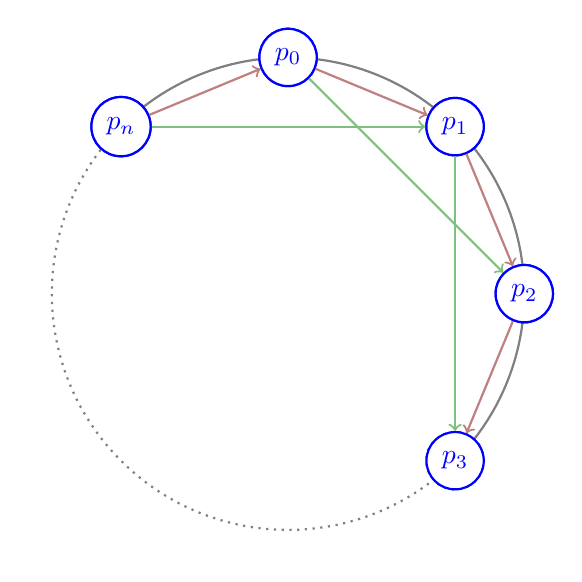
\begin{tikzpicture}
	[ thick,
	  core/.style={draw,circle,blue,fill=white}, 
	  ring/.style={gray},
	  dots/.style={ring,dotted},
	  inner/.style={->},
	  key/.style={font=\small} ]
	
	\draw[ring] node[core] (p0) {$p_0$} (0,0) arc (90:135:3cm) node[core] (pn) {$p_n$};
	\draw[dots] (pn) arc (135:315:3cm) node[core] (p3) {$p_3$};
	\draw[ring] (p3) arc (315:360:3cm) node[core] (p2) {$p_2$};
	\draw[ring] (p2) arc (0:45:3cm) node[core] (p1) {$p_1$};
	\draw[ring] (p1) arc (45:90:3cm) ;
	\node[core] at (p0) {$p_0$};
	\node[core] at (p1) {$p_1$};
	\node[core] at (p2) {$p_2$};
	\node[core] at (p3) {$p_3$};
	\node[core] at (pn) {$p_n$};
	
	\draw[inner,red!50!black!50] (pn) -- node[right,key] {} (p0);
	\draw[inner,red!50!black!50] (p0) -- node[right,key] {} (p1);
	\draw[inner,red!50!black!50] (p1) -- node[right,key] {} (p2);
	\draw[inner,red!50!black!50] (p2) -- node[right,key] {} (p3);
	
	\draw[inner,green!50!black!50] (pn) -- node[left,key] {} (p1);
	\draw[inner,green!50!black!50] (p0) -- node[left,key] {} (p2);
	\draw[inner,green!50!black!50] (p1) -- node[left,key] {} (p3);
	
\end{tikzpicture}

%\end{document}
}
	\caption{Busy ping-pong\index{busy ping-pong} for the first two epochs}
	\label{fig:busypingpong}
\end{figure}

These watchdogs have the following properties (for a stable ring with $n$ peers):
\begin{itemize}
	\item Within period $1/f$ each peer is pinged by some other peer.
	\item Within period $n/f$ each peer has contacted all of the others.  
		This is important in order to have a recent view on the number of files in the memory caches. 
		For 6\,000 peers and 20\,Hz a ``round trip'' takes 5 minutes.
	\item Withing $n-1$ consecutive epochs, we find no duplicate ping-pong-relationship, \ie we constantly change ``who is observing whom''.
\end{itemize}

Pings are not synchronized during an epoch.
This brings an automatic \indexed{jitter}, \ie we avoid that all the peers start to talk on the line at the same time.
After some time the epoch counters of the peers are likely to become out of sync.
Therefore, we adjust the slower peers to the faster ones by skipping epochs.
For instance, if a peer gets a ping with epoch 10, but has itself epoch 8, it immediately switches to 11.

\subsubsection{Network Traffic}
Just by ping-pong messages we produce the following network traffic for $n$ peers and frequency~$f$:
\[ nf(2(\text{MAC header} + \text{IP header} + \text{UDP header}) + \text{ping payload} + \text{pong payload}) \]
which is (for IPv4)
\[ 2nf(18 +  20 + 8 + 9) \text{B} =  110nf \text{B}. \]
For 250 peers and 20\,Hz this turns out to be 4.4\,mbit/s.

\subsubsection{Robustness Analysis}\index{robustness}
We look how fast the peer tables reflect a sudden loss of a number of arbitrary peers. 
We measure the ``recovery speed'' in the number of \indexed{heartbeat}s.
At start, let $n$ the number of peers, \ie each peer has $n$ entries in its table.
At a certain point $rn$ peers fail, $0<r<1$.

Now we have $(1-r)n$ living peers, each of them still having $n$ records in their peer table.
Within the next couple of heartbeats, living peers which happen to ping a failed peer will tell the crowd about the loss.
That means, within the next couple of heartbeats the number of records in the peer tables of the living peers decreases as well as the number of undetected failed peers.
We give an estimation for waiting time until all failed peers are detected.
To do so, we reduce the problem to the \emph{coupon's collector} problem~\cite{feller68}\index{coupon's collector problem}, \ie we calculate the expected total number of pings $\E(P)$.
Knowing that each heartbeat consists of $(1-r)n$ pings, for the expected number of heartbeats $W$ we have
\[ \E(W) = \frac{1}{(1-r)n}\E(P). \]

We assume a randomized setting, in which the processes of ``ping'' are independent Bernoulli experiments.
We calculate the probability for detecting the $i$th failed peer, provided that $i-1$ failed peers are already detected:
\[ p_i = \frac{rn-i+1}{n-i+1}. \]
The expected number of pings for a success $w_i$ is $\E(w_i) = 1/p_i$.
Hence we have
\begin{align*}
	\E(W) &= \frac{1}{(1-r)n}(\E(w_1) + \cdots + \E(w_{rn})) = \frac{1}{(1-r)n}\sum_{i=0}^{rn-1}\frac{n-i}{rn-i} \\
		&\leq \frac{1}{1-r}H_{rn} \approx \frac{\ln(rn)}{1-r}
\end{align*}
The same method estimates the variance using $\sigma^2(w_i)=(1-p_i)/p_i^2$:
\begin{align*}
	\sigma^2(W )&=\frac{\sigma^2(w_1)+\cdots+\sigma^2(w_{rn})}{((1-r)n)^2} = \frac{1}{((1-r)n)^2}\sum_{i=0}^{rn-1}\frac{(1-r)n(n-i)}{(nr-i)^2} \\
		& \leq \frac{1}{(1-r)}\sum_{i=0}^{rn-1}\frac{1}{(nr-i)^2} \leq \frac{\pi^2}{6(1-r)} \leq \frac{2}{1-r}
\end{align*}

Overall we expect a very fast decrease of undetected failed peers.
The theoretical consideration is backed up with simulation results for up to $n=6000$ peers with 64 runs for each combination $n, f=1,\dots,n-1$.
Random variables are the start epoch and the particular failing peers.
Simulation results are shown in Table~\ref{tab:simpingpong}.
\begin{table}
	\begin{center}
		\footnotesize
		\begin{tabular}{|c|cc|cc|cc|}\hline
			\multirow{2}{*}{\backslashbox{Heartbeats}{Peers}} & \multicolumn{2}{c|}{250} & \multicolumn{2}{c|}{1000} & \multicolumn{2}{c|}{2500} \\
				& avg & max & avg & max & avg & max \\ \hline
			$\geq 4$ & 38 & 59 & 42 & 62 & 45 & 62 \\
			$\geq 8$ & 16 & 22 & 18 & 23 & 19 & 23 \\
			$\geq 16$ & 7 & 9 & 8 & 9 & 8 & 9 \\
			$\geq 32$ & 3 & 4 & 4 & 4 & 4 & 4 \\
			\hline
		\end{tabular}
	\end{center}
	\caption{Percentage of cases with high number of heartbeats}
	\label{tab:simpingpong}
\end{table}


\subsubsection{Net Split}\index{net split}
By sending false \msgname{Ciao} messages, we can trigger a net split.
This means we may end up in a stable state where certain sub sets of peers remain with a consistent, but partial view on the crowd.

For example: we have 4 peers, $p_1, \dots, p_4$, increasingly ordered on the ring.
The next epoch is 1.
Consider this sequence (we assume, that a pinging peer is added to the pinged peer's table):
\begin{enumerate}
	\item $p_1$ is declared dead
	\item $p_4$ pings $p_2$
	\item $p_2$ is declared dead
	\item $p_1$ pings $p_3$
	\item $p_3$ is declared dead
	\item $p_2$ pings $p_4$
	\item $p_4$ is declared dead
	\item $p_3$ pings $p_1$  
\end{enumerate}
Now we have two separated crowds, $p_1, p_3$ and $p_2, p_4$.

A slow but sure approach is for each peer to send a \msgname{Moin} message from time to time anyways (\msgname{Alive} message).
This can be combined with the ping so that each peer sends additionally an \emph{Alive} with probability $1/(c\cdot \text{size}(\text{PeerTable}))$.
With every $c$th heartbeat we have an unnecessary multicast \msgname{Moin} (for every sub crowd).

The net split is easily detectable with the first peer that sends to the multicast address.
So as a fast ``\indexed{rejoin}'' mechanism, when a peer from sub crowd $A$ sends its \msgname{Alive}, all the peers from sub crowd $B$ react with a multicast \msgname{Moin} instead of a unicast \msgname{Moin}.
This way, a net split recovers approximately after $c/f$ time (independently from the number of sub crowds).
